%!TEX root = ../presentation.tex

\chapter{Rust Introduction}
\label{chap_rv}
\targets{
  \item Know different approaches and concepts of programming languages, especially memory management.
  \item Get to know the system programming language Rust.
  \item Understand Rust's key concepts, ownership.
}

\section{Rust}

\subsection{What is Rust?}

\begin{Frame}{System Programming Language}
  \begin{Definition}[System programming language]
    A \emph{system programming language} is a programming language used for \alert{system programming}.
  \end{Definition}

  \pause

  \begin{Definition}[System programming]
    \emph{System programming} is the activity of programming \alert{system software}.
  \end{Definition}

  \pause

  \begin{Definition}[System software]
    \emph{System software} is computer software designed to provide a platform to other software.
  \end{Definition}

  \pause

  \begin{exampleblock}{System software}
    Operating systems like macOS and Windows, computational science software, game engines, industrial automation, software as a service applications, \ldots.
  \end{exampleblock}
\end{Frame}

\begin{Frame}[t]{System Programming Language}{Examples}
  \vskip5ex

  \begin{columns}[t]
    \column{0.4\textwidth}
    \inhead{Not System Languages}
    \begin{itemize}
      \item Bash
      \item Python
      \item JavaScript
      \item Java
      \item C\#
      \item \textcolor{gray}{Go}
      \item \textcolor{gray}{Pascal}
      \item \ldots
    \end{itemize}

    \column{0.4\textwidth}
    \inhead{System Languages}
    \begin{itemize}
      \item Assembler
      \item PL/I
      \item C
      \item C++
      \item \alert{Rust}
      \item \textcolor{gray}{Swift}
      \item \textcolor{gray}{Pascal}
      \item \textcolor{gray}{Go}
      \item \ldots
    \end{itemize}
  \end{columns}
\end{Frame}

\begin{Frame}{Type Checking vs.~Testing}
  \inhead{Less Typing}
  \begin{itemize}
    \item Dynamic type checking at runtime
    \item Implicit type conversions
    \item Program faster (rapid prototyping)
    \item Fighting with runtime errors
    \item Many trivial unit tests
  \end{itemize}

  \xxx

  \inhead{More Typing}
  \begin{itemize}
    \item Static type checking at compile time
    \item Complex constraints encoded in type
    \item Once the type fits, the program works
    \item Fighting with the type checker
    \item Less trivial (unit) testing
    \item \alert{Rust: Borrow checker}
  \end{itemize}
\end{Frame}
  
\subsection{Hello, world!}

\begin{Frame}[fragile]{Hello, world!}
  \begin{lstlisting}[language=Rust,gobble=4]
    fn main() {
        println!("Hello, world!");
    }
  \end{lstlisting}

  \xxx

  \begin{lstlisting}[gobble=4]
    $ rustc main.rs
    $ ./main
    Hello, world!
  \end{lstlisting}
\end{Frame}

\begin{Frame}[fragile]{Data Types, Functions, and Control Flow}
  \begin{lstlisting}[language=Rust,gobble=4]
    fn foo(x: i32) -> i32 {
        if x % 2 == 0 {
            x / 2
        } else {
            x * 3 + 1
        }
    }

    fn main() {
      let x = 2.0; // f64
      let y: f32 = 3.0; // f32
      let x = foo(5); // => 16
    }
  \end{lstlisting}
\end{Frame}

\begin{Frame}{The Book}
  \begin{thebibliography}{10}
    \bibitem{RustBook}
    Nicholas Matsakis and Aaron Turon.
    \newblock The Rust Programming Language,
    \newblock \url{https://doc.rust-lang.org/book/}
  \end{thebibliography}

  \vskip5ex

  \tiny
  \begin{columns}
    \column{7.5cm}
    \alert{3. Common Programming Concepts}\\
    \alert{\qquad 3.1. Variables and Mutability}\\
    \alert{4. Understanding Ownership}\\
    \alert{\qquad 4.1. What is Ownership?}\\
    \alert{\qquad 4.2. References \& Borrowing}\\
    \qquad 4.3. Slices\\
    \alert{10. Generic Types, Traits, and Lifetimes}\\
    \qquad 10.1. Generic Data Types\\
    \qquad 10.2. Traits: Defining Shared Behavior\\
    \alert{\qquad 10.3. Validating References with Lifetimes}\\
    \alert{15. Smart Pointers}\\
    \alert{\qquad 15.1. Box Points to Data on the Heap and Has a Known Size}\\
    \qquad 15.4. Rc, the Reference Counted Smart Pointer\\
    \qquad 15.5. RefCell and the Interior Mutability Pattern\\
    19. Advanced Features\\
    \qquad 19.1. Unsafe Rust\\
  \end{columns}
\end{Frame}

\subsection{Mutability}

\lstset{basicstyle=\ttfamily\scriptsize}

\begin{Frame}[fragile]{Immutability is the Default}
  \begin{lstlisting}[language=Rust,gobble=4]
    fn main() {
        let x = 5;
        println!("The value of x is: {}", x);
        x = 6; // ERROR!
        // cannot assign twice to immutable variable `x`
        println!("The value of x is: {}", x);
    }
  \end{lstlisting}
\end{Frame}

\begin{Frame}[fragile]{Explicit Mutability}
  \begin{lstlisting}[language=Rust,gobble=4]
    fn main() {
        let mut x = 5;
        println!("The value of x is: {}", x);
        x = 6;
        println!("The value of x is: {}", x);
    }
  \end{lstlisting}
\end{Frame}

\begin{Frame}[fragile]{Shadowing}
  \begin{lstlisting}[language=Rust,gobble=4]
    fn main() {
        let x = 5;

        let x = x + 1;

        let x = x * 2;

        println!("The value of x is: {}", x);
    }
  \end{lstlisting}
\end{Frame}

\begin{Frame}[fragile]{Shadowing With Different Types}
  \inhead{Mutable Variable Has Fixed Typed}
  \begin{lstlisting}[language=Rust,gobble=4]
    let mut spaces = "   ";
    spaces = spaces.len(); // ERROR!
    // mismatched types
  \end{lstlisting}

  \vskip5ex
  
  \inhead{Shadowing Can Introduce New Type}
  \begin{lstlisting}[language=Rust,gobble=4]
    let spaces = "   ";
    let spaces = spaces.len();
  \end{lstlisting}
\end{Frame}

\lstset{basicstyle=\ttfamily}

\section{Memory Management}

\subsection{Manual}

\begin{Frame}[fragile]{Pointers in C}
  \begin{lstlisting}[language=C,gobble=4]
    // Declare a variable
    int var = 23;

    // Declare pointer variable 
    int *ptr; 
    
    // Assign the address of var to ptr
    ptr = &var;

    // Read var through the pointer
    printf("%d\n", *ptr); // => 23

    // Write var through the pointer
    *ptr += 19;

    // Read var
    printf("%d\n", var); // => 42
  \end{lstlisting}
\end{Frame}

\begin{Frame}[fragile]{Pointers to Arrays}
  \begin{lstlisting}[language=C,gobble=4]
    // Declare an array and a pointer variable
    int arr[3] = {42, 23, 4223};
    int *ptr;
  
    // Assign the address of arr[0] to ptr
    ptr = arr;

    // Read arr through the pointer
    for (int i = 0; i <= 3; i++) 
    { 
        printf("ptr = %p\n", ptr);
        printf("*ptr = %d\n\n", *ptr);
  
        // Increment pointer ptr by 1 
        ptr++; 
    }
  \end{lstlisting}
\end{Frame}

\begin{Frame}[fragile]{Pointers to Arrays}{Output}
  \begin{lstlisting}[gobble=4]
    ptr = 0x7ffee481b91c
    *ptr = 42
    
    ptr = 0x7ffee481b920
    *ptr = 23
    
    ptr = 0x7ffee481b924
    *ptr = 4223
    
    ptr = 0x7ffee481b928
    *ptr = -1285554006
  \end{lstlisting}
\end{Frame}

\begin{Frame}[fragile]{Malloc \& Free}
  \begin{lstlisting}[language=C,gobble=4]
    // Request memory for dynamic array
    int* ptr = malloc(5 * sizeof(int));

    // Initialize memory
    for (int i = 0; i < 5; i++)
        ptr[i] = i;

    // Use memory
    // ...

    // Free memory
    free(ptr);
  \end{lstlisting}
\end{Frame}

\begin{Frame}[fragile]{Stack \& Heap}
  \begin{lstlisting}[language=C,gobble=4]
    int* empty() {
        int* result = malloc(3 * sizeof(int));
        for (int i = 0; i < 3; i++)
            result[i] = i;
        return result;
    }

    int main() {
        int i = 12;
        int *ptr = empty();
        for (int i = 0; i < 3; i++)
            printf("%d\n", ptr[i]);
        free(ptr);
    }
  \end{lstlisting}
\end{Frame}

\begin{Frame}{Stack \& Heap}
  \centerline{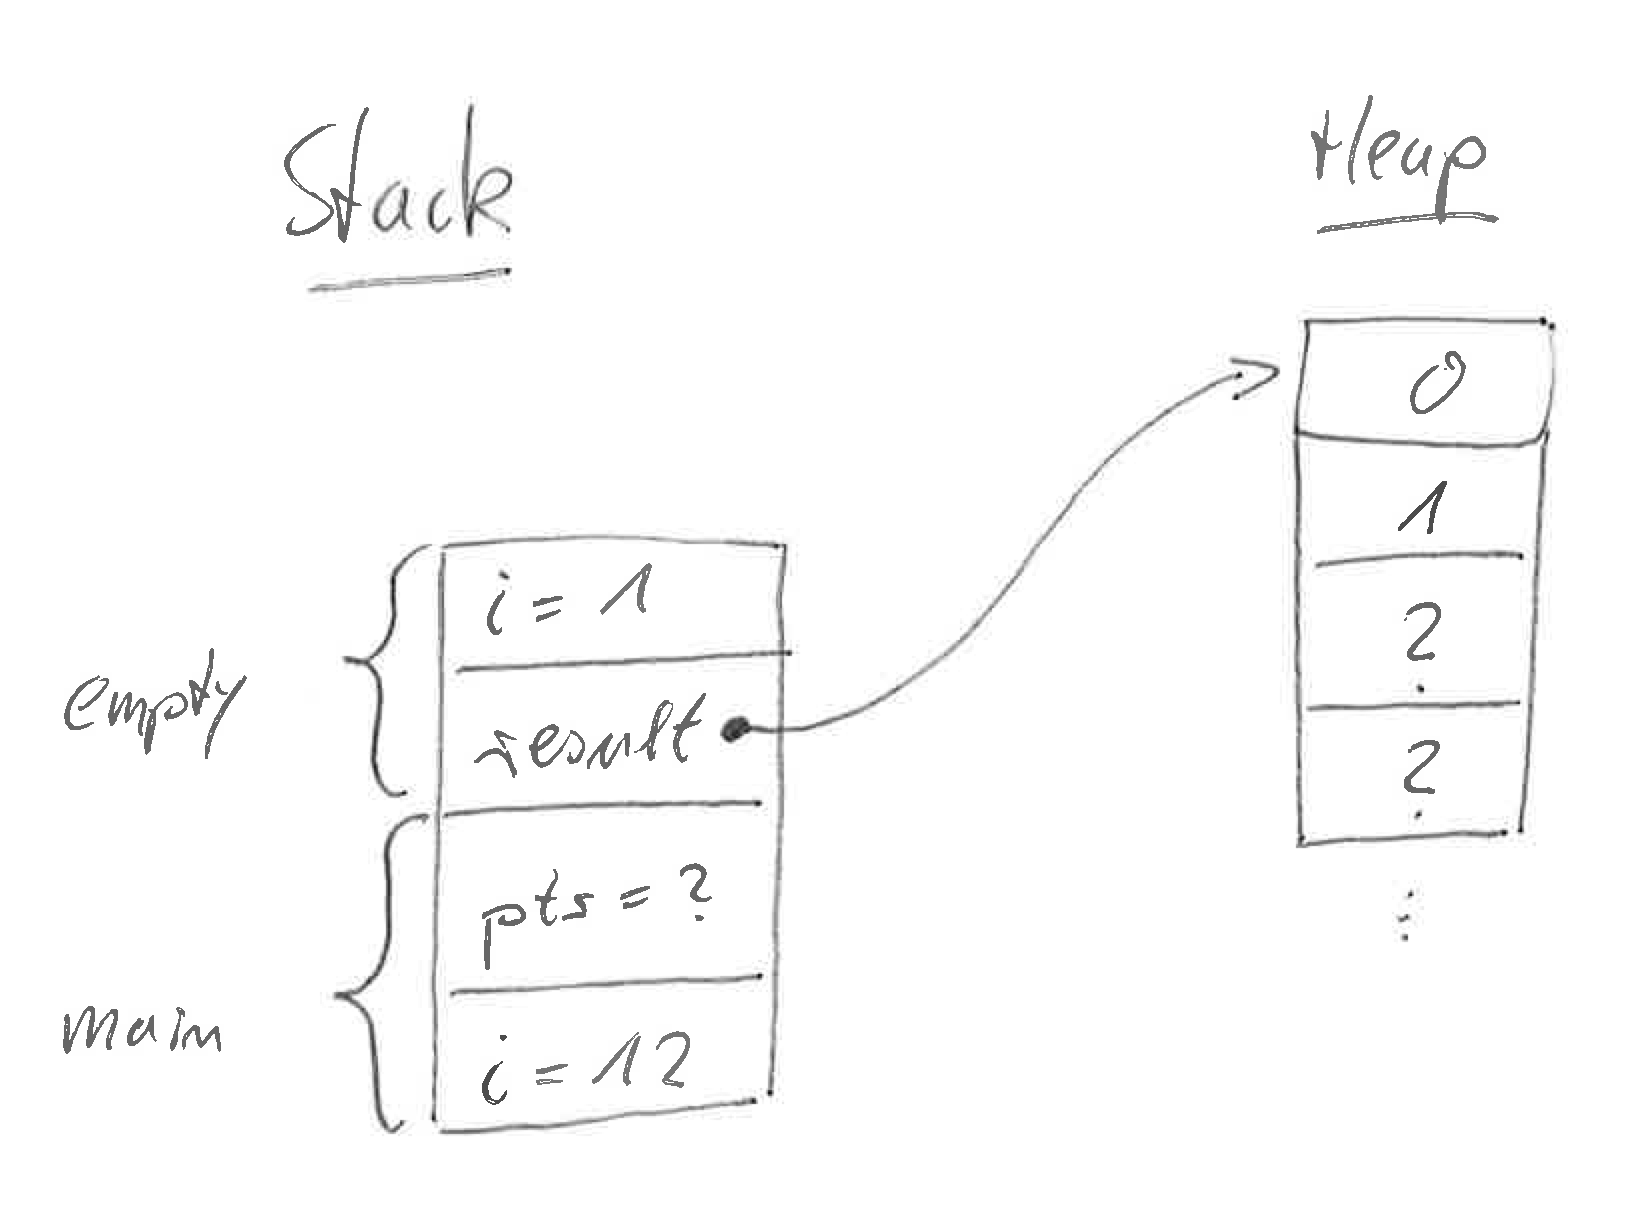
\includegraphics[width=8cm]{content/chapter_rust/stack+heap}}
\end{Frame}


\subsection{Reference Counting}

\begin{Frame}[plain]{Reference Counting (Objective C / Swift)}
  \textwidthplain
  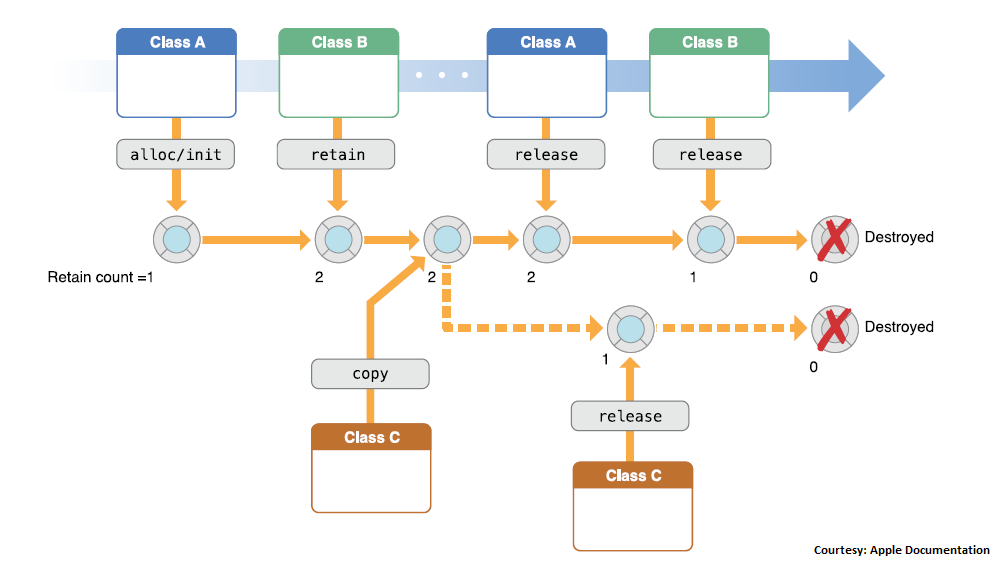
\includegraphics[width=\textwidth]{content/chapter_rust/memorymgnt_objectivec.png}
\end{Frame}

\begin{Frame}{Reference Counting (Objective C / Swift)}
  \begin{itemize}
    \item NSObject provides reference counting
    \item Manual Retain-Release Basic Rules
      \begin{itemize}
        \item We own any object we create
        \item We can take ownership of an object using retain
        \item When we no longer need it,\\
          we must relinquish ownership of an object we own
      \end{itemize}
    \item Automatic Reference Counting
      \begin{itemize}
        \item Same reference counting in NSObject used
        \item Compiler inserts memory management method calls\\
          for us at compile-time
        \item Sometimes called \enquote{static garbage collection}
      \end{itemize}
  \end{itemize}
\end{Frame}

\subsection{Tracing Garbage Collecting}

\begin{Frame}[fragile]{Important Terms of Garbage Collecting}
  \begin{Definition}[Unreachable objects]
    An object is said to be \emph{unreachable}\\ iff it doesn't contain any available reference to it.
  \end{Definition}

  \begin{lstlisting}[language=Java,gobble=4]
    Integer i = new Integer(4);
    // Integer object reachable via i
    i = null;
    // Integer object no longer reachable
  \end{lstlisting}

  Note that objects which are part of an \alert{island of isolation}\\
  are also unreachable.

  \begin{Definition}[Eligibility for garbage collection]
    An object is said to be eligible for garbage collection\\ iff it is unreachable.
  \end{Definition}
\end{Frame}

\begin{Frame}{Garbage Collection}
  \begin{itemize}
    \item Memory is allocated but never freed by the user.
    \item Runtime environment periodically stops program and\\
      frees memory of objects eligible for garbage collection.
    \item User cannot control when garbage collection runs.\\
      Java's \texttt{System.gc()} is only a request.
  \end{itemize}

  \xxx

  \begin{exampleblock}{Question}
    Are memory leaks possible with garbage collection?
  \end{exampleblock}
\end{Frame}

\begin{Frame}{Garbage Collection (GC) Algorithms}
  \begin{description}
    \item[Mark-and-Sweep] Stop program,\\
      Mark everything reachable from the GC roots,\\
      free every non-marked object.
    \item[Compacting GC] Defragment memory after\\
      freeing the unreachable objects.
    \item[Copying GC] Stop program, Copy everything reachable from the GC roots to new heap, discard old heap.
    \item[Parallel GC] Search in parallel.
    \item[Concurrent GC] Search and free without stopping.\\
      \emph{Stop needed for finding roots and compacting.}
    \item[Generational GC] Young Spaces: Copying GC,\\
      Old Spaces: Mark-and-Sweep.
  \end{description}
\end{Frame}

\begin{Frame}{Should I use Garbage Collection?}
  \inhead{Pros}
  \begin{itemize}
    \item Easier to use, rapid programming
    \item Less error-prone
  \end{itemize}
  \xxx

  \inhead{Cons}
  \begin{itemize}
    \item Maybe slower
    \item Pauses, less real-time
    \item Less control
  \end{itemize}
  \xxx

  \pause
  \inhead{Conclusion}
  \begin{itemize}
    \item It depends!
  \end{itemize}
\end{Frame}

\section{Ownership in Rust}

\subsection{What is Ownership?}

\lstset{basicstyle=\ttfamily\scriptsize}

\begin{Frame}[fragile]{Variable Scope}
  \begin{lstlisting}[language=Rust,gobble=4]
    // s is not valid here, it's not yet declared
    {                      
        // s is valid from this point forward
        let s = "hello";

        // do stuff with s
    }
    // this scope is now over, and s is no longer valid
  \end{lstlisting}
\end{Frame}

\begin{Frame}[fragile]{Mutable Strings}
  \begin{lstlisting}[language=Rust,gobble=4]
    // string literal, where value is hardcoded
    let s = "hello";

    // Immutable string
    let s = String::from("hello");

    // Mutable string
    let mut s = String::from("hello");

    // push_str() appends a literal to a String
    s.push_str(", world!"); 

    println!("{}", s); // => hello, world!
  \end{lstlisting}
\end{Frame}

\begin{Frame}[fragile]{Memory and Allocation}
  \begin{lstlisting}[language=Rust,gobble=4]
    {
        // s is valid from this point forward
        // => allocate memory for value
        let s = String::from("hello"); 

        // do stuff with s
    }
    // this scope is now over, and s is no longer valid
    // => free memory, Rust calls s.drop()
  \end{lstlisting}

  \begin{block}{Note}
    In C++, this pattern of deallocating resources at the end of
    an item's lifetime is sometimes called \emph{Resource Acquisition
    Is Initialization (RAII)}. The drop function in Rust will be
    familiar to you if you've used RAII patterns.
  \end{block}
\end{Frame}

\begin{Frame}[fragile,t]{Ways Variable and Data Interact: Move}
  \begin{lstlisting}[language=Rust,gobble=4]
    let s1 = String::from("hello");
    let s2 = s1;

    println!("{}, world!", s1); // ERROR!
  \end{lstlisting}

  \hskip3cm
  \only<2>{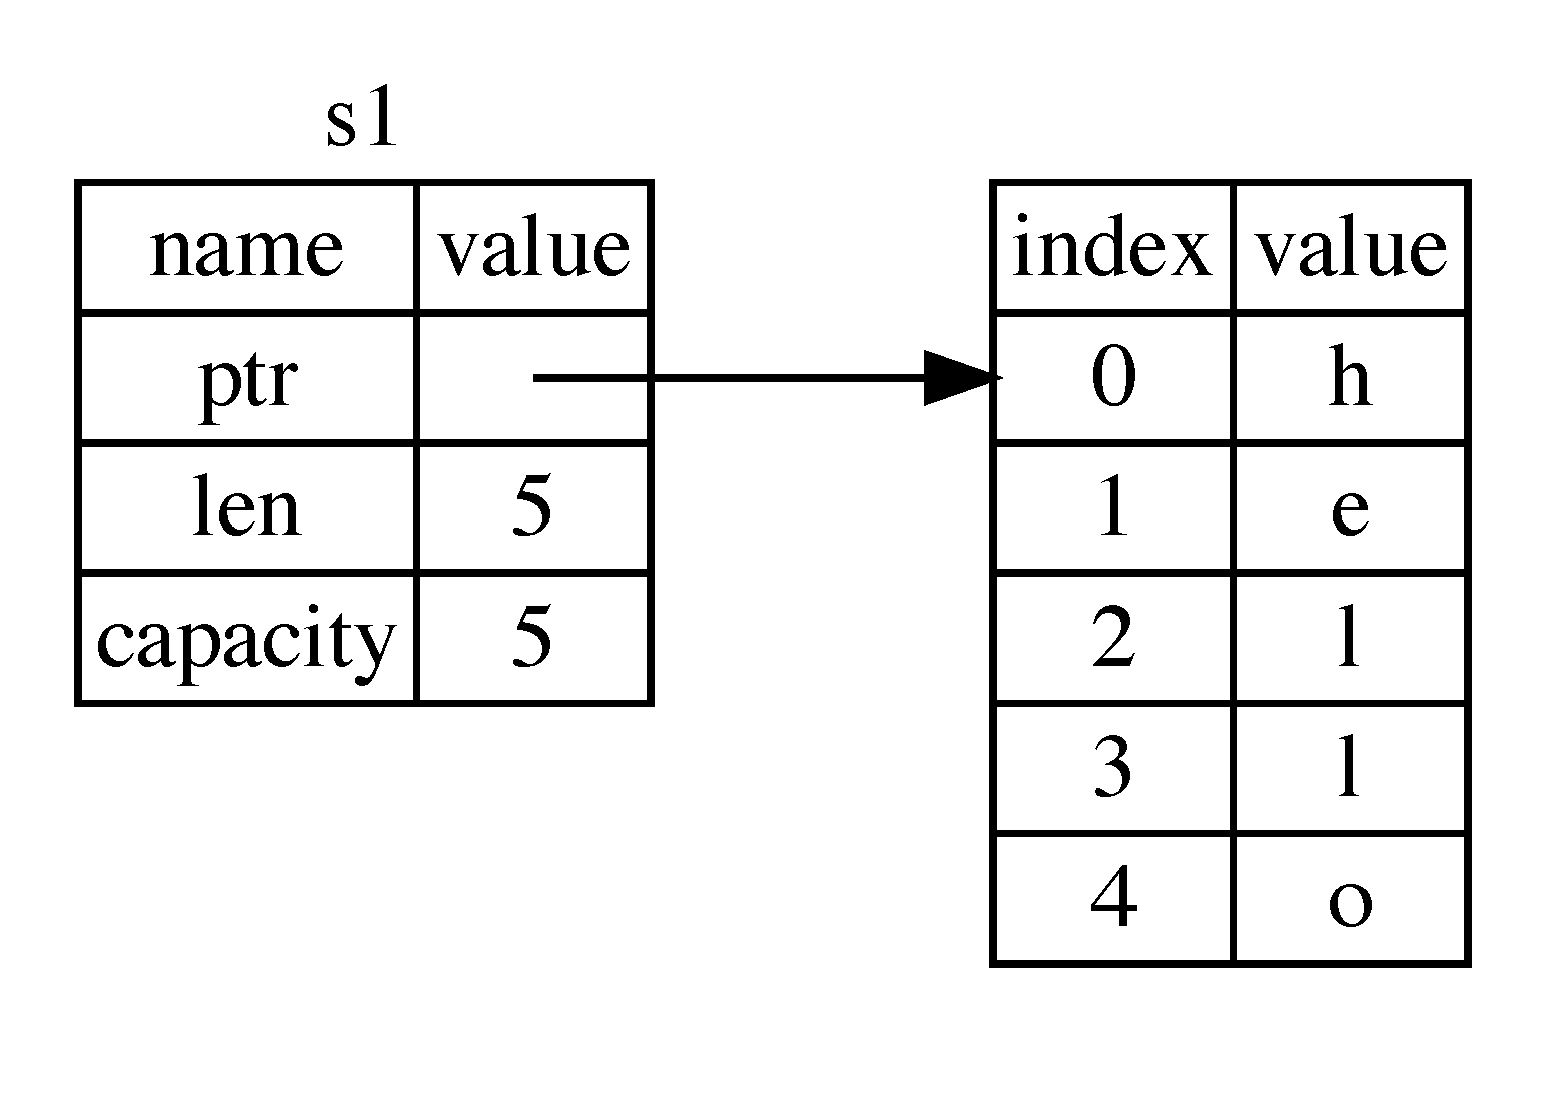
\includegraphics[width=4cm]{content/chapter_rust/rust-move-01}}%
  \only<3>{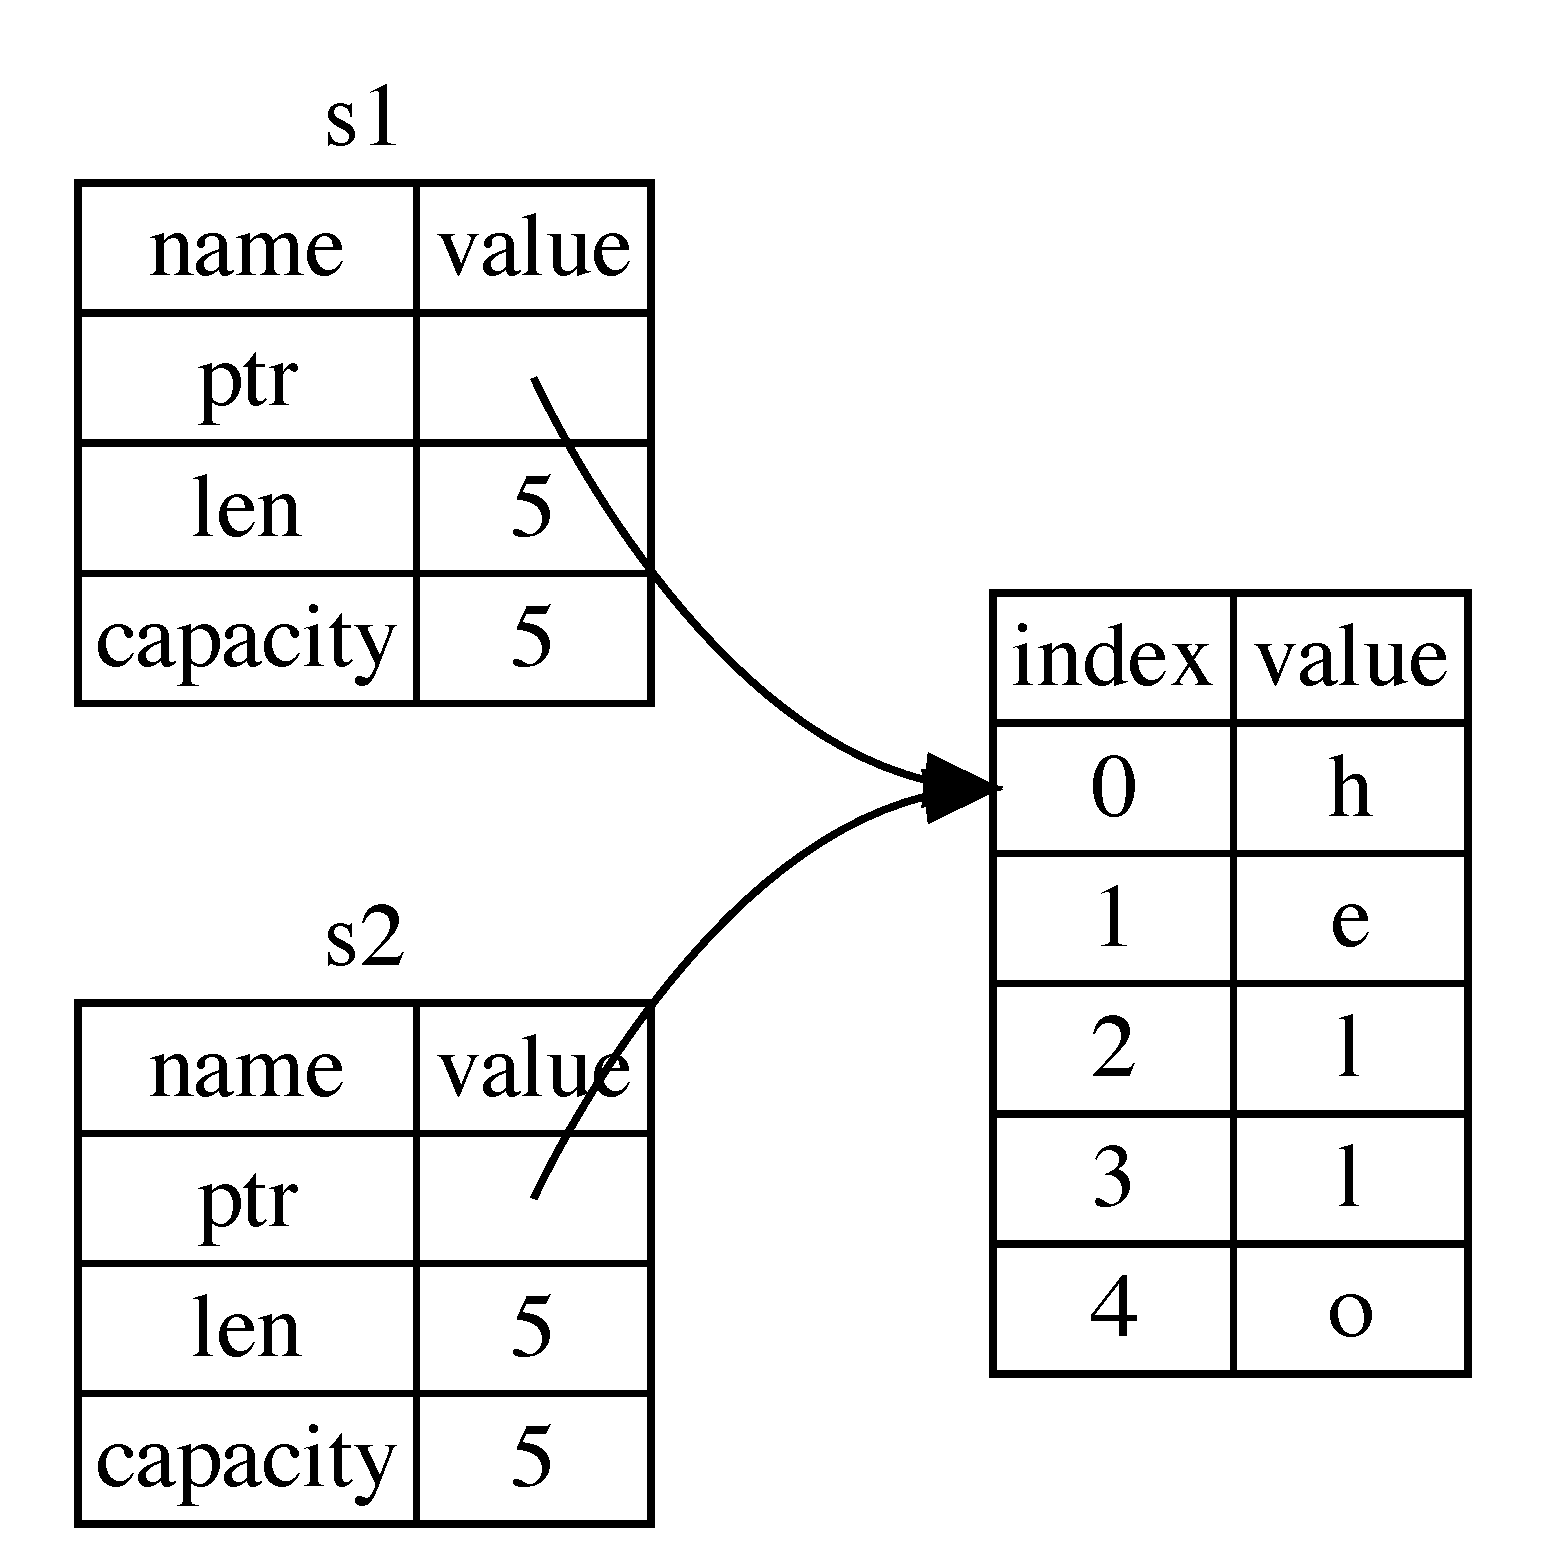
\includegraphics[width=4cm]{content/chapter_rust/rust-move-02}}%
  \only<4>{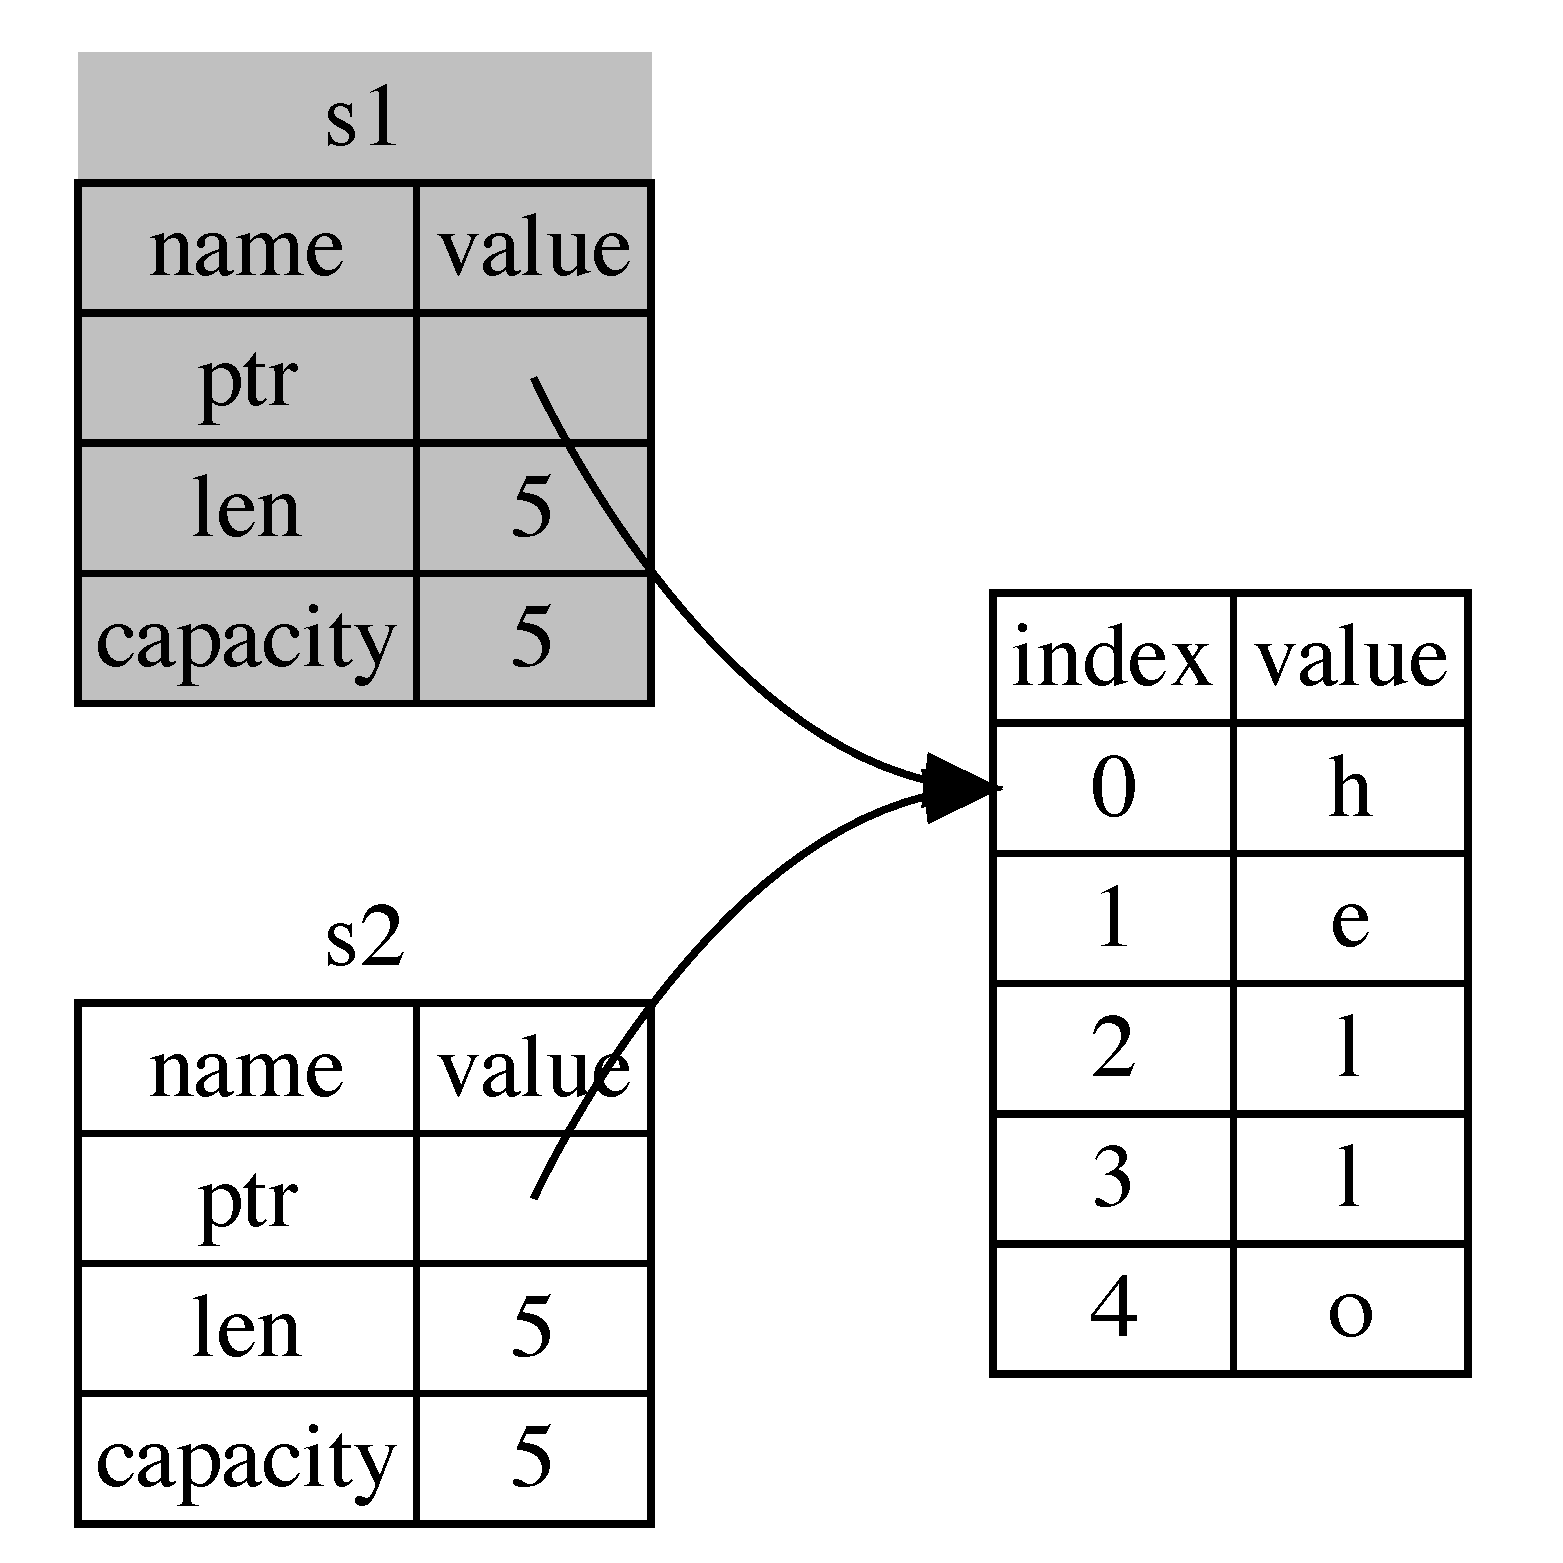
\includegraphics[width=4cm]{content/chapter_rust/rust-move-03}}
\end{Frame}

\begin{Frame}[fragile,t]{Ways Variables and Data Interact: Clone}
  \begin{lstlisting}[language=Rust,gobble=4]
    let s1 = String::from("hello");
    let s2 = s1.clone();

    println!("s1 = {}, s2 = {}", s1, s2);
  \end{lstlisting}

  \hskip3cm
  \only<2>{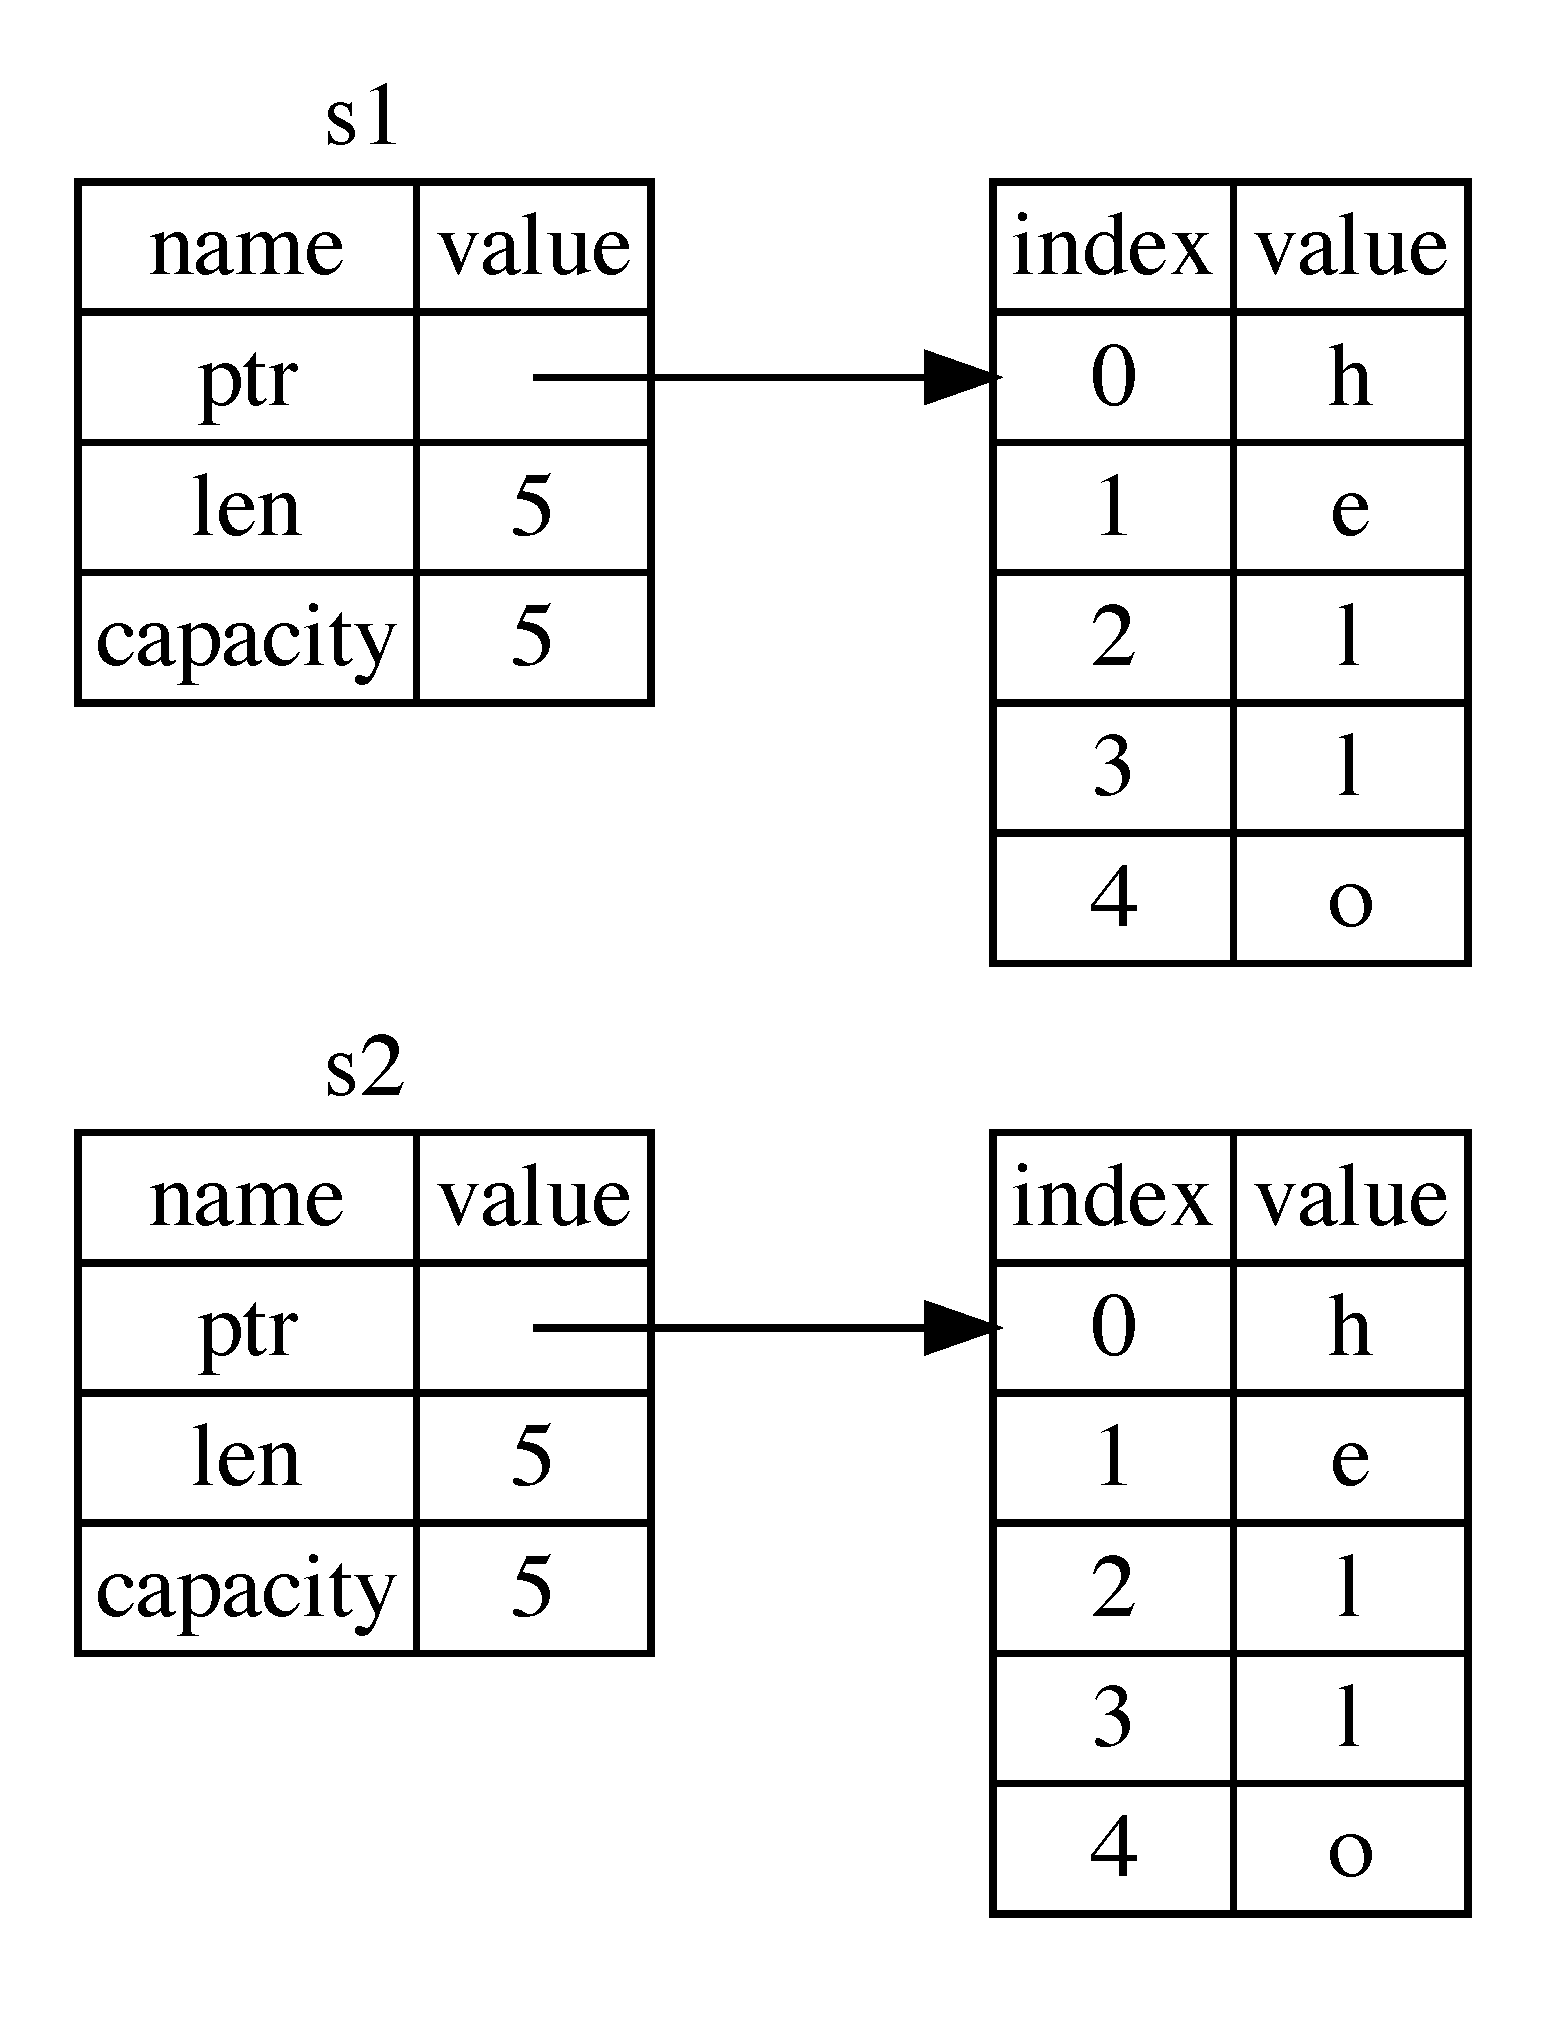
\includegraphics[width=4cm]{content/chapter_rust/rust-copy}}
\end{Frame}

\begin{Frame}{Move vs. Clone}
  \Large\centering
  \alert{Rust's design choice}: Rust will \alert{never automatically} create \alert{deep
    copies} of your data. Therefore, any \alert{automatic copying} can be
  assumed to be \alert{inexpensive} in terms of runtime performance.
\end{Frame}

\begin{Frame}{Stack-Only Data: Copy}
  \begin{itemize}
    \item For primitive data types: deep copy = shallow copy.
    \item Hence, they are always cloned and never moved.
    \item Primitive data types are annotate with the \texttt{Copy} trait.
    \item A data type cannot implement both,\\
      \texttt{Copy} trait and \texttt{Drop} trait.\\
      \alert{Either you mange memory or you are \texttt{Copy}.}
  \end{itemize}
\end{Frame}

\begin{Frame}[fragile,plain]{Ownership and Functions}
  \textwidthplain
  \lstset{basicstyle=\ttfamily\fontsize{6.8pt}{6.8pt}\selectfont,frame=none,backgroundcolor={}}
  \begin{lstlisting}[language=Rust,gobble=4]
    fn main() {
        let s = String::from("hello");  // s comes into scope

        takes_ownership(s);             // s's value moves into the function...
                                        // ... and so is no longer valid here

        let x = 5;                      // x comes into scope

        makes_copy(x);                  // x would move into the function,
                                        // but i32 is Copy, so it's okay to still
                                        // use x afterward

    } // Here, x goes out of scope, then s. But because s's value was moved, nothing
      // special happens.


    fn takes_ownership(some_string: String) { // some_string comes into scope
        println!("{}", some_string);
    } // Here, some_string goes out of scope and `drop` is called. The backing
      // memory is freed.


    fn makes_copy(some_integer: i32) { // some_integer comes into scope
        println!("{}", some_integer);
    } // Here, some_integer goes out of scope. Nothing special happens.
  \end{lstlisting}
\end{Frame}

\begin{Frame}[fragile,plain]{Return Values and Scope}
  \textwidthplain
  \lstset{basicstyle=\ttfamily\fontsize{6.8pt}{6.8pt}\selectfont,frame=none,backgroundcolor={}}
  \begin{lstlisting}[language=Rust,gobble=4]
    fn main() {
        let s1 = gives_ownership();         // gives_ownership moves its return
                                            // value into s1

        let s2 = String::from("hello");     // s2 comes into scope

        let s3 = takes_and_gives_back(s2);  // s2 is moved into
                                            // takes_and_gives_back, which also
                                            // moves its return value into s3
    } // Here, s3 goes out of scope and is dropped. s2 goes out of scope but was
      // moved, so nothing happens. s1 goes out of scope and is dropped.


    fn gives_ownership() -> String {             // gives_ownership will move its
                                                 // return value into the function
                                                 // that calls it

        let some_string = String::from("hello"); // some_string comes into scope

        some_string                              // some_string is returned and
                                                 // moves out to the calling
                                                 // function
    }


    // takes_and_gives_back will take a String and return one
    fn takes_and_gives_back(a_string: String) -> String { // a_string comes into
                                                          // scope

        a_string  // a_string is returned and moves out to the calling function
    }
  \end{lstlisting}
\end{Frame}

\subsection{References and Borrowing}

\begin{Frame}[fragile,t]{Passing Values Without Loosing Ownership}{Return Ownership Afterwards}
  \begin{lstlisting}[language=Rust,gobble=4]
    fn main() {
        let s1 = String::from("hello");

        let (s2, len) = calculate_length(s1);

        println!("The length of '{}' is {}.", s2, len);
    }

    fn calculate_length(s: String) -> (String, usize) {
        let length = s.len();

        (s, length)
    }
  \end{lstlisting}
\end{Frame}

\begin{Frame}[fragile,t]{Passing Values Without Loosing Ownership}{Better: Pass a Reference}
  \begin{lstlisting}[language=Rust,gobble=4]
    fn main() {
        let s1 = String::from("hello");

        let len = calculate_length(&s1);

        println!("The length of '{}' is {}.", s1, len);
    }

    fn calculate_length(s: &String) -> usize {
        s.len()
    }
  \end{lstlisting}

  \pause

  \only<2>{\centerline{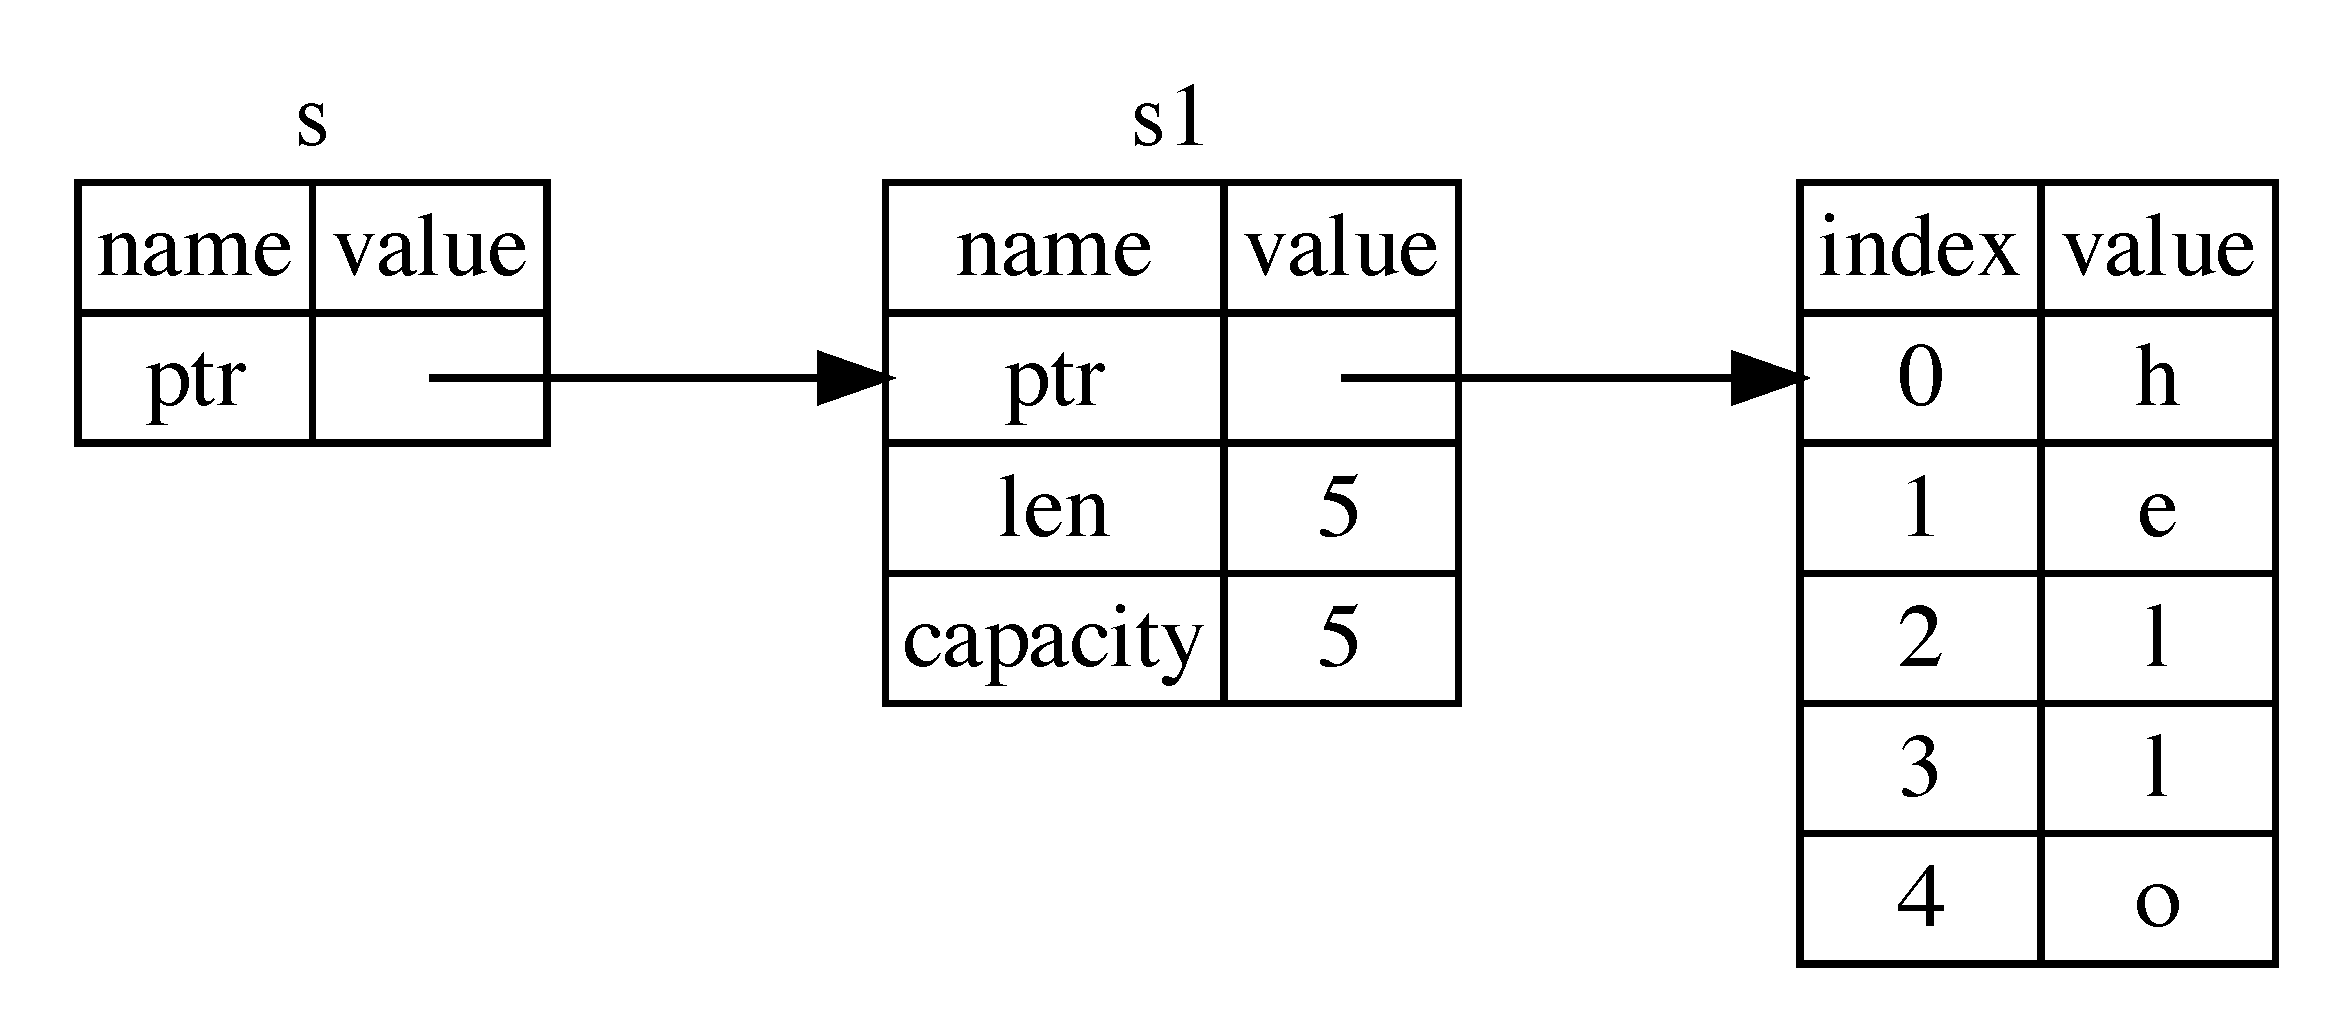
\includegraphics[width=7cm]{content/chapter_rust/rust-reference}}}
  \only<3>{\begin{Definition}[Borrowing]
    We call having references as function parameters \emph{borrowing}.
  \end{Definition}
   As in real life, if a person owns something, you can borrow it from them. When you're done, you have to give it back.}
\end{Frame}

\subsection{Mutable References}

\begin{Frame}[fragile,t]{References are Immutable}
  \begin{lstlisting}[language=Rust,gobble=4]
    fn main() {
        let s = String::from("hello");

        change(&s);
    }

    fn change(some_string: &String) {
        some_string.push_str(", world"); // ERROR!
        // cannot borrow immutable borrowed content
        // `*some_string` as mutable
        // 
    }
  \end{lstlisting}
\end{Frame}

\begin{Frame}[fragile,t]{Mutable References}
  \begin{lstlisting}[language=Rust,gobble=4]
    fn main() {
        let mut s = String::from("hello");

        change(&mut s);
    }

    fn change(some_string: &mut String) {
        some_string.push_str(", world");
    }
  \end{lstlisting}
\end{Frame}

\begin{Frame}[fragile]{You Can Have Only One Mutable Reference}
  \begin{lstlisting}[language=Rust,gobble=4]
    let mut s = String::from("hello");

    let r1 = &mut s;
    let r2 = &mut s; // ERROR!
    // cannot borrow `s` as mutable
    // more than once at a time

    println!("{}, {}", r1, r2);
  \end{lstlisting}
\end{Frame}

\section*{Conclusion}

\begin{frame}{Conclusion}
  \begin{enumerate}
    \item \alert{Rust} is a \alert{modern system programming languages} with many safety features build in the \alert{strong static type checking}.
    \item There are different \alert{memory management strategies} (manual, reference counting, garbage collecting, ownership and borrowing, \ldots). It is \alert{up to you to} decide what you need!
    \item \alert{Ownership} in Rust: For every memory object there is \alert{exactly one owner}.
    \item \alert{References} in Rust: At any given time, you can have \alert{either one mutable reference or any number of immutable references}. References must always be valid.
  \end{enumerate}
\end{frame}
